\documentclass[]{tRSL2e}

%\documentclass[journal]{IEEEtran}
%\documentclass[a4paper, 10pt, conference]{ieeeconf}

\usepackage{graphicx}
\usepackage{pstricks}

\def\row{10}
\def\column{10}

\usepackage{xcolor}
\definecolor{plot}{rgb}{0,0.0964,1.00}

\newsavebox\IBox
\savebox\IBox{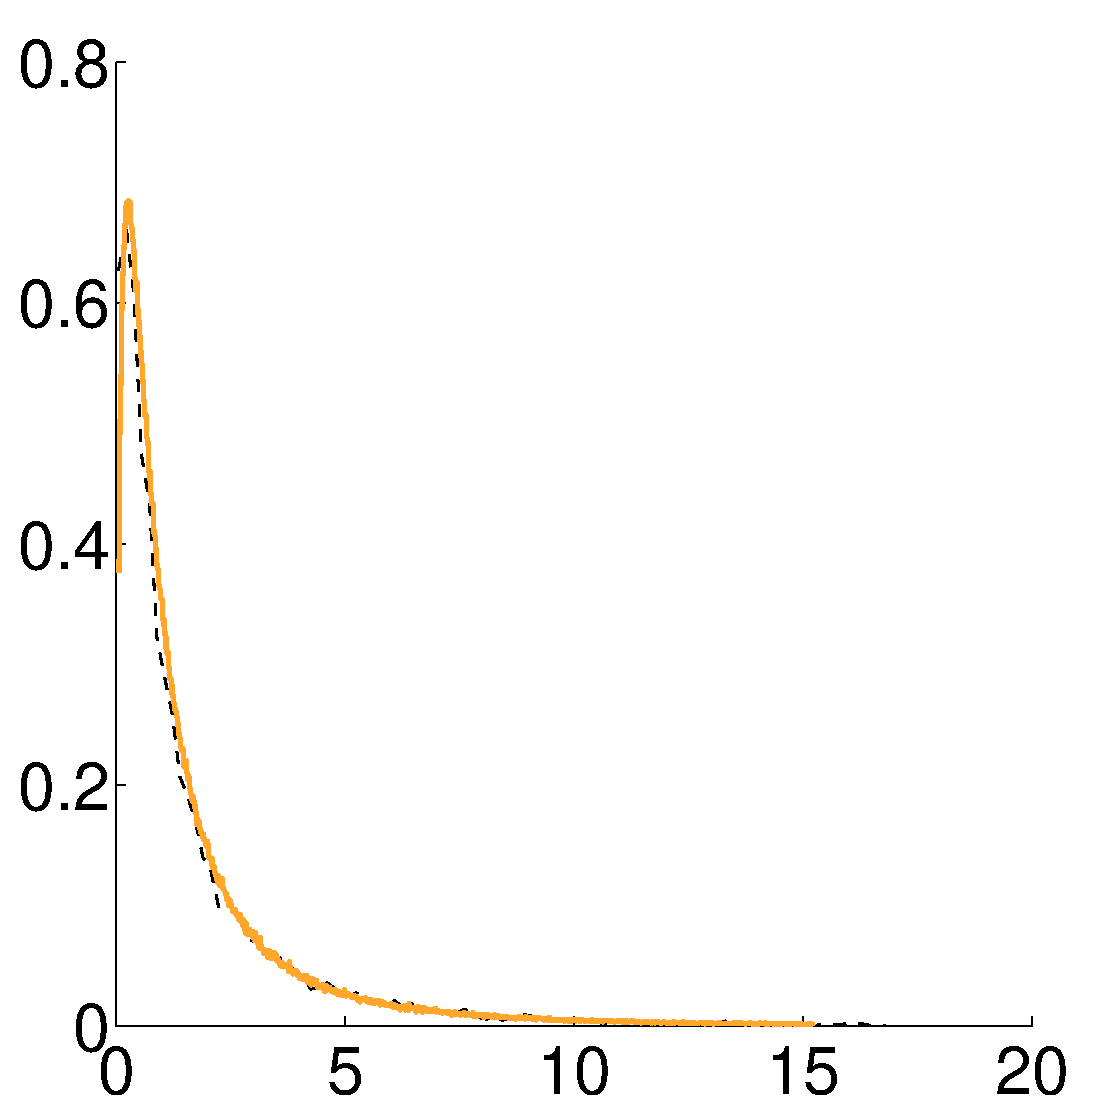
\includegraphics[width=1.5in,height=1.5in]{../images/verify_change_ratio_model_on_RADARSAT2_3d.eps}}

\psset
{
  xunit=\dimexpr\wd\IBox/\column,
  yunit=\dimexpr\ht\IBox/\row,
}

\newcommand{\plotWithLegend}[2]{          
          \begin{pspicture}[showgrid=false](\column,\row)% set showgrid=false for the final
	    \rput[bl](0,0){\includegraphics[width=1.5in,height=1.5in]{#1}}% \usebox\IBoxCRThreeR
	    %\rput(5,1.5){\footnotesize{#2}}
	    %\rput{90}(1.5,5){\footnotesize{pdf / histogram}}
	    \psline[linecolor=plot](5,8)(6,8)
	    \psline[linestyle=dashed](5,9)(6,9)%another line style: dotted
	    \rput(8,8){model}
	    \rput(8,9){data}            
          \end{pspicture}
}

\usepackage{cite} %for citations
\renewcommand{\citedash}{--}
\usepackage{url}

 %this is for math typing (eg: cases)
\usepackage{amsmath}
   \usepackage{amsfonts}   % if you want the fonts
   \usepackage{amssymb}    % if you want extra symbols
\usepackage{epsfig} %for figures

\usepackage[center]{caption}%for captions
\usepackage{subcaption}
%\usepackage[caption=false,font=scriptsize]{subfig} %for subfigures

%opening
\title{
  Scalar and Representative Observables for Polarimetric SAR Data
}



\begin{document}

\author{
  Thanh-Hai~Le$^{\ast}$$\dag$\thanks{$^\ast$Corresponding
author. Email: le\_thanh\_hai@hotmail.com \vspace{6pt}},
  and Ian~McLoughlin${\ddag}$, 
  and Chan-Hua~Vun${\dag}$\\
\vspace{6pt} $\dag$School of Computer Engineering, Nanyang Technological University, Singapore.\\
$\ddag$ University of Science and Technology of China.\\
\vspace{6pt}\received{November 2013} }

\maketitle

\begin{abstract}
%Problem statement  
This paper proposes a scalar and representative observable for multi-dimensional POLSAR data,
  from which statistically consistent discrimination measures can be derived.
%What actually were done? and As the result, what is learned?
Specifically, the statistical behaviour of the POLSAR covariance matrix determinant is used
  to derive a scalar and generic statistical model for multi-dimensional POLSAR data,
  which is specifically applicable to the two and three dimensional versions of partial and full monostatic polarimetric SAR data.
As the POLSAR covariance matrix determinant generalizes the SAR intensity towards multiple dimensions,
  the proposed model is able to subsume the traditional SAR intensity model under the umbrella of a unified model. 
%What are the larger implications of the findings presented in this paper?
Consequently, the main beneficial implication of the proposed approach is that
  it provides a consistent theory unifying the currently disconnected proposals for SAR and POLSAR discrimination measures
  which simplifies the adaptation of existing SAR data processing techniques for POLSAR data.
%  it enables the adaptation of many existing SAR data processing techniques for POLSAR data,
%  and at the same time, it provides a consistent theory unifying the seemingly disparate discrimination measure proposals for SAR and POLSAR data.
\end{abstract}


\section{Introduction}

%What is the situation, the background context of your research? the BIG problem!
Relentless growth in computing power has allowed once computationally-demanding Synthetic Aperture Radar (SAR)
to become a feasible and preferred technique for earth observation.
Basic SAR has also been extended in a few directions, one of which is polarimetric SAR (POLSAR).
This exploits the natural polarization property of Electro-Magnetic (EM) waves,
  encoded in multiple channels, compared to traditional one-channel SAR.
  

%Research Motivation: Why it is important to solve this problem?
%The POLSAR data, however, is multidimensional and stochastic.
POLSAR data, like SAR, is stochastic but is also multi-dimensional, making it even harder to interpret.
It is therefore important to establish a simple and intuitive understanding of the data.
 Statistical models are undoubtedly crucial in understanding its stochastic nature.
While several %multidimensional 
models have been proposed for POLSAR data, they
   tend to be complex and unintuitive due to the multidimensional nature of the data.
Practical POLSAR data processing however, makes heavy use of scalar discrimination measures,
  which should be based on statistically consistent models %for scalar and representative observables 
  of the multidimensional data.
It is thus important to establish scalar and representative observables for multi-dimensional POLSAR data.
  
%Moreover, to provide theoretical foundation for discrimination measures proposal,
%  statistically consistent models should be derived from this scalar observable.

%How do others solve this problem?
%The complex POLSAR data have been statistically modelled as following the complex Wishart distribution,
%  which apparently is multidimensional, complex and thus not very intuitive.
A few scalar POLSAR observables with accompanying statistical models have been proposal \citep{Conradsen_2003_TGRS_4, Alberga_2008_IJRS_4129, Joughin_1994_TGRS_562, Lee_1994_TGRS_1017, Touzi_1996_TGRS_519, Lopez-Martinez_2003_TGRS_2232, Erten_2012_Sensors_2766},
  but none is able to provide meaningful scalar discrimination measures.
%  but none of them has led to scalar discrimination measures proposal.
As such no observable has been widely accepted as being highly representative of this multi-dimensional data,
  which severely limits their applicability in practical data processing applications.
Alternatively, a few POLSAR discrimination measures have been proposed,
  but all based on likelihood ratio statistics.
This should ideally be based on an exact and consistent distribution
  but so far only asymptotic distributions have been demonstrated.

%Research Objective: Give your precise problem statement  
This article presents a scalar and representative observable, and its associated generic statistical model, to describe multi-dimensional POLSAR data and provide a consistent foundation for the derivation of discrimination measures.
%Now State your approach  
%This study started off with the observation that the determinant of the covariance matrix is widely used in POLSAR discrimination measures.
%However, our survey of existing scalar models for POLSAR indicates that no statistical model for this observable has been published so far.
%Consequently, in this article, the statistical behaviour of the determinant of POLSAR covariance matrix is further investigated.
%Prof Vuns: comment: the article provides the result, not the journey!
POLSAR data have been statistically modelled as following the complex Wishart distribution.
Consequently, the generic statistical model for the covariance matrix determinant is presented as being just a scalar projection of the multidimensional data.
This model is then used to derive several scalar and consistent statistical descriptions suggesting that their associated observables are capable of being used as discrimination measures for POLSAR.
%
%***IVM: the following sentence doesn't make sense, also, I don't think it's good to talk about 'models of a model'.  Maybe 'model variants' instead?
%%%***IVM***The specific two and three dimensional models of these models, which %also include the derived discrimination measures, are originally designed against both partial and full polarimetric SAR data.

%The specific two and three dimensional models are then validated against both partial and full polarimetric SAR data.
We will also show that %It is also shown that
  the specific one dimensional (1-D) versions of the proposed  models 
  match %perfectly with 
  the traditional statistical model used for SAR intensity.
This effectively incorporates SAR theory under the umbrella of the proposed scalar approach for multi dimensional POLSAR.
The different discrimination proposals for SAR and POLSAR are reviewed in light of this and the  proposed in this paper is shown to provide a strong, unifying and consistent foundation. % relating them all together.
The applicability of these theoretical models will be illustrated by experiments where the specific 1, 2 and 3-D versions of the proposed models are validated against practical data. 
%Furthermore, the approach proposed in this paper
%  not only provides a consistent foundation for the different discrimination measures proposal in POLSAR
%  but also leads to the establishment of a new discriminating measures: the determinant-ratio and the change-ratio.

%What is the novelty of your solution? What are its advantages
%Compared to other published scalar observables with accompanying statistical model,
%  the proposed observable and its models are highly representative of the multidimensional data.
%The representative power of the proposed observable is justified by the following reasons.
%Firstly, the covariance matrix determinant, when collapsed into one-dimensional case, transforms neatly into the representative SAR intensity.
%Secondly, the statistical model for this observable is shown as the generic multi-dimensional extension of the traditional and representative intensity model for the one dimensional SAR data.
%And last but not least, this observable also leads to the determinant-ratio discrimination measure which
%  not only is simpler in concept and computation than the existing POLSAR discrimination measures
%  but also can be considered as the natural multi-dimensional extension of the commonly-used intensity-ratio discrimination measure in SAR.
% Prof Vun Comment: already mentioned above, no need to repeat
%hai thoughts: actually this should be included to justify our title, and our approach. It is however being moved to discussion / conclusion section

%How do you know if the problem is solved? State your research contribution to be achieved
%In summary, the main objective of this article is to propose the determinant of the POLSAR covariance matrix as a scalar observable
%  that is representative of the multi-dimensional data.
%Specifically the following research results are to be achieved:
%  1. The generic scalar and representative statistical model for the determinant of the multi-dimensional POLSAR covariance matrix is to be derived, 
%  2. This generic model is also shown leading to staititically consistent models for newly proposed POLSAR observables, namely the determinant-ratio and the change-ratio.
%  3. The special one-dimensional version of the derived generic model is to be shown perfectly matches with the traditionally used SAR intensity model,
%  4. All specific one, two and three dimensional versions of the derived generic model are to be validated against real-life captured data,
%(Hai NOTE: I kept this to keep my focus while working on this paper.
%  It can be removed before the final submission.)
  
%Article Organization: Show that you deliver on the objectives and hence solve the stated problem

%%***IVM SKIP THIS TO SAVE SPACE - letters usually don't have this
%The remainder of this article is organized as follows.
%After the next section reviews existing discrimination measures as well as scalar observables models for POLSAR, section \ref{sec:theoretical_model}
%  derives the generic statistical model for the determinant of the POLSAR covariance matrix
 % and proposes several new discrimination measures for the multi-dimensional data.
%After section \ref{sec:sar_special_case_of_polsar} illustrates the match between the specific model of one dimensional and the traditional model for SAR intensity,
 % section \ref{sec:link_sar_polsar} links the disparate discrimination measure proposals for the traditional SAR and the more recent POLSAR data.
%The applicability of these models against practical data is illustrated in section \ref{sec:polsar_models_validation}.
%Section \ref{sec:discussion} presents a high-level discussion of the results presented before
 % section \ref{sec:conclusion} finally concludes the paper.
  
\section{Related Work in Literature}
\label{sec:lit_review}

%Section \ref{sec:lit_models} reviews various statistical models used for different scalar observables for POLSAR.
%  where it is shown that none are able to provide statistically consistent discrimination measures. 
%Section \ref{sec:lit_measures} further strengthens those findings by discussing discrimination measures that have been proposed for POLSAR,
 % and demonstrates that almost all of them are based on the likelihood statistical test for complex Wishart distribution.
%While an exact statistical distribution is expected to be necessary for a test,
 % only an asymptotic distribution is used in the underlying approach \citep{Conradsen_2003_TGRS_4}.
  
%**IVM save space!
%\subsection{Scalar Observables for POLSAR Data and their Statistical Models}
%\label{sec:lit_models}

Different target decomposition theorems have identified many possible scalar observables for complex POLSAR data.
\citet{Alberga_2008_IJRS_4129} evaluated the performance of different scalar POLSAR observables for classification.
While many were presented, their corresponding statistical models and classifiers were not available.
Furthermore, the paper concluded that it is impossible to identify a single best representation.
Although, to be fair, the observables were identified for describing a decomposed portion of the complex POLSAR data,
  rather than a unified representation.
%
Using a different approach, given that the joint distribution for POLSAR is known to be the multi-variate complex Wishart,
  it is possible to derive the scalar statistical models for some univariate POLSAR observables.
%This becomes an alternative approach used in the study of POLSAR data.
However, this is non-trivial -- so far, only a handful of such models have been proposed, including:
  \begin{enumerate}
  \item cross-pol ratio $r_{HV/HH} = |S_{HV}|^2/|S_{HH}|^2$ \citep{Joughin_1994_TGRS_562},
  \item co-pol ratio $r_{VV/HH} = |S_{VV}|^2/|S_{HH}|^2$ \citep{Joughin_1994_TGRS_562},
  \item co-pol phase difference $\phi_{VV/HH} = arg(S_{VV}S_{HH}^*) $ \citep{Joughin_1994_TGRS_562} \citep{Lee_1994_TGRS_1017},
  \item magnitude $g=|avg(S_{pq}S_{rs}^*)|$ \citep{Lee_1994_TGRS_1017},
  \item normalized magnitude $\xi = \frac{|avg(S_{pq}S_{rs}^*)|}{\sqrt{avg(|S_{pq}|^2) avg(|S_{rs}|^2)}}$ \citep{Lee_1994_TGRS_1017},
  \item intensity ratio $w = avg(|S_{pq}|^2)/avg(|S_{rs}|^2)$ \citep{Lee_1994_TGRS_1017},
  \item and the Stokes parameters $S_i,0 \leq i \leq 3$ \citep{Touzi_1996_TGRS_519}. 
  \end{enumerate}
More recently, statistical models for
  each element of the POLSAR covariance matrix, i.e. $S_{pq}S_{rs}^*$, \citep{Lopez-Martinez_2003_TGRS_2232}
  as well as for the largest eigen-value of the covariance matrix $\lambda_1$ \citep{Erten_2012_Sensors_2766} have been proposed. Although useful, these have not been shown to result in statistically consistent discrimination measures or 
 be representative of the complex POLSAR data.
%While these models undoubtedly help to further our understandings of the POLSAR data,
 % none of the underlying observables have been shown to meet the dual criteria of
 % 1) resulting in statistically consistent discrimination measures and thus 
 % 2) being representative of the complex POLSAR data.

\subsection{POLSAR Discrimination Measures}
\label{sec:lit_measures}

Euclidean or Manhattan distance measures for matrices are not widely used 
for POLSAR due to the multiplicative nature of the noise.
%, defined respectively as:
%\begin{align}
%  d(C_x,C_y) &= \sum_{i,j} |\mathbb{R} (C_x - C_y)_{i,j}| + \sum_{i,j} |\mathbb{I} (C_x - C_y)_{i,j}| \\
%  d(C_x,C_y) &= \sqrt{\sum_{i,j} |C_x - C_y|_{i,j}^2 }
%\end{align}
%where $C_{i,j}$ denotes the $(i,j)$ elements of the POLSAR covariance matrix C,
% $||$ denotes absolute values
%and $\mathbb{R},\mathbb{I}$ denote the real and imaginary parts respectively.
Instead, the Wishart distance is probably most common, as part of the well-known Wishart classifier \citep{Lee_1999_TGRS}, defined \citep{Lee_1994_IJRS_2299} as:
$d(C_x,C_y) = \ln|C_y| + tr(C_xC_y^{-1})$
where $tr(C)$ denotes the trace of the POLSAR covariance matrix C. 
As a measure of distance, its main disadvantage is that $d(C_y,C_y) = \ln|C_y| \neq 0$.

Recent works have suggested alternative dissimilarity measures including the symmetric and asymmetric refined Wishart distance \citep{Anfinsen_2007_ESA_POLINSAR},
\vspace{-2mm}
\begin{align}
  d(C_x,C_y) &= \frac{1}{2} tr(C_x^{-1}C_y + C_y^{-1}C_x) - d \\
    d(C_x,C_y) &= \ln|C_x| - \ln|C_y| + tr(C_xC_y^{-1}) - d
\end{align}
\vspace{-2mm}
the Bartlett distance \citep{Kersten_2005_TGRS_519},
     \vspace{-2mm}
  \begin{align}
  d(C_x,C_y) &= 2 \ln |C_{x+y}| - \ln |C_x| - \ln |C_y| - 2d\ln2
  \end{align}
     \vspace{-2mm}
the Bhattacharyya distance \citep{Lee_2011_IGARSS_3740},
     \vspace{-2mm}
\begin{equation}
  r(C_x,C_y) = \frac{|C_x|^{1/2} |C_y|^{1/2}}{|(C_x+C_y)/2|}
\end{equation}
     \vspace{-2mm}
and the Wishart Statistical test distance \citep{Cao_2007_TGRS_3454},
     \vspace{-2mm}
\begin{equation}
  d(C_x,C_y) = (L_x + L_y) \ln|C| - L_x \ln|C_x| - L_y\ln|C_y|
\end{equation}

Closer examination of these reveal that most are related:
The Bhattacharyya and Bartlett distances are easily shown to be related.
At the same time, Barlett can be considered a special case of the Wishart Statistical Test distance,
  when the two data sets have the same number of looks, i.e. $L_x=L_y$.
The close relation among  measures may be due to the fact that
  all of their publications refer to, and are based on, the same statistical model in \citep{Conradsen_2003_TGRS_4}.
In \citep{Conradsen_2003_TGRS_4}, to determine if the two scaled multi-look POLSAR covariance matrixes $Z_x$ and $Z_y$,
  which have $L_x$ and $L_y$ as the corresponding number of looks,
  come from the same underlying stochastic process,
the likelihood ratio statistics for POLSAR covariance matrix is considered:  
     \vspace{-2mm}
\begin{equation}
  Q = \frac{(L_x+L_y)^{d \cdot (L_x+L_y)}}{L_x^{d \cdot L_x} L_y^{d \cdot L_y}} \frac{|Z_x|^{L_x} |Z_y|^{L_y} }{|Z_x+Z_y|^{(L_x+L_y)}}
\end{equation}

Taking the log-transformation of the above equation, and denoting $C_{vx} = Z_x / L_x$, $C_{vy} = Z_y / L_y$ and $C_{vxy} = (Z_x + Z_y)/(L_x + L_y)$ then:
{\small
\begin{align}
  Q &= \frac{|C_{vx}|^{L_x} \cdot |C_{vy}|^{L_y} }{|C_{vxy}|^{L_x + L_y}} \label{eqn:ori_likelyhood_stats} \\
  \ln Q &= L_x \ln |C_{vx}| + L_y \ln |C_{vy}| - (L_x + L_y) \ln |C_{vxy}| \label{eqn:log_likelyhood_stats}
\end{align}
}
\vspace{-2mm}

To detect changes, a test statistic is developed for this discrimination measure.
i.e. a distribution is derived for the dissimilarity measure.
However, \citet{Conradsen_2003_TGRS_4} only use an asymptotic distribution.
By contrast, this paper proposes a statistical model for the determinant of the POLSAR covariance matrix $|C_v|$
  which is capable of providing an exact distribution for the test.

\section{The Generic Scalar Statistical Model for POLSAR}  
\label{sec:theoretical_model}

In this section, the generic scalar statistical model for POLSAR is presented.
%In this section, after the basic foundations of POLSAR statistical analysis are introduced,
 % the generic scalar statistical model for the multi-dimensional POLSAR will be presented.
%  this section presents the theoretical model for multi-dimensional POLSAR data. 
%
%In this paper, the POLSAR scattering vector is denoted as $s$.
%For partial polarimetric SAR (single polarization in transmit and dual polarization in receipt),
%  the vector is two-dimensional ($d=2$) and is normally written as: 
%\begin{equation}
%s_{part}=\begin{bmatrix}
%S_h\\ 
%S_v
%\end{bmatrix}
%\end{equation}
%For full and monostatic POLSAR data,
 % the vector is three-dimensional ($d=3$) and is presented as:
%\begin{equation}
%s_{full}=\begin{bmatrix}
%S_{hh}\\
%\sqrt{2}S_{hv}\\
%S_{vv}
%\end{bmatrix}
%\end{equation}
%
First, let $\Sigma=E [ss^{*T}]$ denote the population expected value of the POLSAR covariance matrix,
  where $s^{*T}$ is the complex conjugate transpose of the POLSAR scattering vector, $s$. 
%Assuming 
If this is jointly circular complex Gaussian with expected covariance matrix $\Sigma$,
  then the PDF of $s$ can be written as
$pdf(s;\Sigma)=\{1/{\pi^d|\Sigma|}\} exp\{-s^{*T}\Sigma^{-1}s\}$
where $||$ denotes the matrix determinant.
%
The sample POLSAR covariance matrix is formed as the mean of Hermitian outer product of independent single-look scattering vectors,
     \vspace{-4mm}
\begin{equation}
  C_v = \langle ss^{*T} \rangle = \frac{1}{L} \sum^L_{i=1}s_is_i^{*T}
\end{equation}
where $L$ is the number of looks
 and $s_i$ denotes the partial or full POLSAR scattering vector respectively.
%
Complex Wishart distribution statistics are normally used for the scaled covariance matrix
$Z=LC_v$, whose PDF is given as:
\begin{equation}
  pdf(Z;d,\Sigma,L)=\frac{|Z|^{L-d}}{|\Sigma^L|\Gamma_d(L)}e^{-tr(\Sigma^{-1}Z)}
\end{equation}
with $\Gamma_d(L) = \pi^{d(d-1)/2} \prod^{d-1}_{i=0}\Gamma(L-i)$
and $d$ the dimension number of the POLSAR covariance matrix.
%
The approach taken in this paper differs by applying a homoskedastic log transformation  on a less-than-well-known relationship.
\citet{Goodman_1963_AMS_178} found
that the ratio between observable and expected values of the sample covariance matrix determinants
  behaves like a product of $d$ chi-squared random variables with different degrees of freedom: 
\vspace{-2mm}
\begin{equation}
\chi^d_L = (2L)^d \frac{|C_v|}{|\Sigma_v|} \sim \prod_{i=0}^{d-1} \chi (2L-2i)
\label{eqn:prod_chi_squared_rv}  
\end{equation}

%We will now use 
We use this to develop a generic scalar statistical model. %log-transformed measures of distance.
From Eqn. \ref{eqn:prod_chi_squared_rv} we have:
\vspace{-2mm}
\begin{eqnarray}
  |C_v| &\sim& |\Sigma_v| \cdot \frac{1}{(2L)^d} \cdot \prod_{i=0}^{d-1} \chi (2L-2i) \label{eqn:determinant_distribution} %\\
%  \ln|C_v| &\sim& \ln|\Sigma_v| - d \cdot \ln(2L) + \sum^{d-1}_{i=0} \Lambda(2L-2i)
%\label{eqn:log_determinant_distribution}  
\end{eqnarray}

Over a homogeneous area, $\Sigma_v$, $d$ and $L$ are considered constant.
Thus Eqn. \ref{eqn:determinant_distribution} indicates that a multiplicative speckle noise pattern is present 
  in the original POLSAR domain.
Moreover, since the average and variance of these chi-squared distributions are %and log-chi-squared distribution
constant, i.e. $avg \left[ \chi(2L) \right] = 2L$ and $var \left[ \chi(2L) \right] = 4L$,
  their product and summation also have fixed summary statistics.
Specifically:
\vspace{-2mm}
{
\begin{align*}
  avg \left[ \prod^{d-1}_{i=0} \chi(2L-2i) \right] &= 2^d \cdot \prod^{d-1}_{i=0} (L-i), \\
  var \left[ \prod^{d-1}_{i=0} \chi(2L-2i) \right] &= \prod^{d-1}_{i=0} 4(L-i)(L-i+1) - \prod^{d-1}_{i=0} 4(L-i)^2, %\\
%  avg \left[ \sum^{d-1}_{i=0} \Lambda(2L-2i) \right] &= d \cdot \ln{2} + \sum^{d-1}_{i=0} \psi^0(L-i), \\
%  var \left[ \sum^{d-1}_{i=0} \Lambda(2L-2i) \right] &= \sum^{d-1}_{i=0} \psi^1(L-i)
\end{align*}
}

Combining these results with Eqn. \ref{eqn:determinant_distribution} %and \ref{eqn:log_determinant_distribution}
  , we have:
\vspace{-2mm}  
%{
%\begin{align}
%  avg \left[ |C_v| \right]  &= \frac{|\Sigma_v|}{L^d} \prod^{d-1}_{i=0} (L-i)\\
%  var \left[ |C_v| \right]  &=   \frac{|\Sigma_v|^2 \left[ \prod^{d-1}_{i=0} (L-i)(L-i+1) - \prod^{d-1}_{i=0} (L-i)^2 \right] }{L^{2d}} \label{eqn:var_det_is_heteroskedastic}%\\
%%  avg \left[ \ln |C_v| \right] &= \ln |\Sigma_v| - d \cdot \ln{L}  + \sum^{d-1}_{i=0} \psi^0(L-i) \label{eqn:avg_log_det} \\
%%  var \left[ \ln |C_v| \right] &=  \sum^{d-1}_{i=0} \psi^1(L-i) \label{eqn:var_log_det_is_homoskedastic}
%\end{align}
%}
{
\begin{align}
  avg \left[ |C_v| \right]  &= \frac{|\Sigma_v|}{L^d} \prod^{d-1}_{i=0} (L-i)\\
  var \left[ |C_v| \right]  &=   {\frac{|\Sigma_v|^2}{L^{2d}}{ \left[ \prod^{d-1}_{i=0} (L-i)(L-i+1) - \prod^{d-1}_{i=0} (L-i)^2 \right] }} 
 \label{eqn:var_det_is_heteroskedastic}%\\
%  avg \left[ \ln |C_v| \right] &= \ln |\Sigma_v| - d \cdot \ln{L}  + \sum^{d-1}_{i=0} \psi^0(L-i) \label{eqn:avg_log_det} \\
%  var \left[ \ln |C_v| \right] &=  \sum^{d-1}_{i=0} \psi^1(L-i) \label{eqn:var_log_det_is_homoskedastic}
\vspace{-5mm}
\end{align}
}


For a real world captured image, while parameters $d$ and $L$ do not change for the whole image,
  the underlying $\Sigma_v$ is likely to differ from one region to the next.
Thus over a heterogeneous scene, the stochastic process for $|C_v|$ and $\ln |C_v|$ vary depending on the underlying signal $\Sigma_v$. 
Eqn. \ref{eqn:var_det_is_heteroskedastic} implies that the variance of $|C_v|$ will also differ depending on the underlying signal $\Sigma_v$ (i.e. it is   heteroskedastic).
Similar to the way intensity-ratio is proposed as the discrimination measure for the multiplicative and heteroskedastic SAR intensity \citep{Rignot_1993_TGRS_896},
this paper proposes the determinant-ratio and the change-ratio as discrimination measures for the POLSAR data.
%  which is shown above to also suffer from the multiplicative and heteroskedastic phenomena.
%Similar to the way dispersion and contrast is defined for one-dimensional SAR \citep{Le_2010_ACRS},
%  this section introduces the consistent sense of distance for POLSAR.

%Assuming, on the one hand,
If the true value of the underlying signal $\Sigma_v$ is known \textit{a priori},
then the determinant-ratio of the signal random variable ($\mathbb{R}_{\Sigma}$) %and log-distance ($\mathbb{L}$)
%  are observable according to the following definitions:
  is defined as:
%Eqns. \ref{eqn:prod_chi_squared_rv} and \ref{eqn:sum_log_chi_squared_rv} lead straight to the definition of the following random variables, which is the :
$\mathbb{R}_{\Sigma} = {|C_v|}/{|\Sigma_v|}$
%On the other hand, under a looser assumption %From another perspective
For POLSAR data from a homogeneous area, but when the true value of $\Sigma_v$ is \textit{unknown},
 then a random variable called the change-ratio $\mathbb{R}_{C}$)  is defined, $ \mathbb{R}_{C} = {|C_1|}/{|C_2|}$ where $C_1$ and $C_2$ are samples of the covariance matrix determinant in an assumed homogeneous area. 
%
%  the dispersion ($\mathbb{D}$) and contrast ($\mathbb{C}$) random variables are the observables defined as:
%\begin{eqnarray}
%  \mathbb{D} &=& \ln{|C_v|} - avg(\ln{|C_v|}) \label{eqn:dispersion_observable}\\
%  \mathbb{C} &=& \ln(|C_{v1}|) - \ln(|C_{v2}|) \label{eqn:contrast_observable}
%\end{eqnarray}
%
Using the results from Eqn. \ref{eqn:determinant_distribution}, %\ref{eqn:log_determinant_distribution} and \ref{eqn:avg_log_det}
  we have
\begin{equation}%\label{eqn:determinant_ratio_distribution}
\mathbb{R}_{\Sigma} \sim \frac{1}{(2L)^d} \cdot \prod_{i=0}^{d-1} \chi (2L-2i)  ~~and~~
\mathbb{R}_{C} \sim \prod_{i=0}^{d-1} \frac{\chi(2L-2i)}{\chi(2L-2i)} \label{eqn:change_ratio_distribution}
\vspace{-5mm}
\end{equation}
%
%with $\Delta(2L) \sim \Lambda(2L) - \Lambda(2L)$
%and $k=\sum^{d-1}_{i=0} \psi^0(L-i)$
%
%Thus the characteristic functions for the summative random variables is derived in Appendix \ref{sec:appendix_b} as:
%\begin{align}
%  CF_{\Lambda^d_L}(t) &= \frac{2^{idt}}{\Gamma(L)^d} \prod^{d-1}_{j=0} \Gamma(L-j+it) \\
%  CF_{\mathbb{L}}(t) &= \frac{1}{L^{idt} \Gamma(L)^d} \prod^{d-1}_{j=0} \Gamma(L-j+it) \\
%  CF_{\mathbb{D}}(t) &= \frac{e^{ikt}}{\Gamma(L)^d} \prod^{d-1}_{j=0} \Gamma(L-j+it) \\
%  CF_{\Delta(2L)} &= \frac{\Gamma(2L) B(L-it,L+it)}{\Gamma(L)^2} \\
%  CF_{\mathbb{C}}(t) &=  \prod^{d-1}_{j=0} \frac{\Gamma(2L-2j) B(L-j-it,L-j+it)}{\Gamma(L-j)^2}
%\end{align}
%
Since each elementary component follows fixed distributions (i.e. $\chi^2(2L)$),
this variable naturally also follows fixed distributions.
Moreover, it is independent of the underlying $\Sigma_v$,
  indicating its statistically consistent properties (i.e. its applicability as a POLSAR discrimination measure).
%This claim is extrapolated from the widely-used intensity-ratio as a SAR discrimination measure
 % and will be further discussed in the next sections.
%is further strengthened in the next section which shows that the generic models for POLSAR presented in this paper also include the commonly-used models for SAR as its special 1-dimensional case. 
%This result shows how
%In short, these random variables are shown to follow consistent and fixed distributions,
%  regardless of the underlying signal $\Sigma_v$.

\section{SAR as a one-dimensional case of POLSAR}
\label{sec:sar_special_case_of_polsar}

%The previous sections have introduced and validated the theoretical models for 3-dimensional ($d=3$) full polarimetric and 2-dimensional ($d=2$) partial polarimetry, cases.
This section shows that the proposed generic model is  applicable to the 1-D case ($d=1$),
physically equivalent to  collapsing the multi-dimensional POLSAR dataset  into single dimensional SAR data.
Mathematically, the sample covariance matrix $C_v$ is reduced to the sample variance while determinant $|C_v|$ becomes the scalar variance.
As variance is equal to intensity $I$ in SAR, our result is consistent with previous results for SAR intensity.
Thus the proposed generic model for POLSAR, collapsed into 1-D will be shown to apply also to traditional SAR intensity.% as a natural case of the unified model.
%  as well as reminding us that SAR is a special case of POLSAR.
  
The results for our models can be summarised using the following equations:
\begin{equation}\nonumber
  |C_v| \sim |\Sigma_v| \cdot \frac{1}{(2L)^d} \cdot \prod_{i=0}^{d-1} \chi (2L-2i) 
\end{equation}
\begin{eqnarray}\nonumber
\mathbb{R}_{\Sigma} = \frac{|C_v|}{|\Sigma_v|} \sim \frac{1}{(2L)^d} \prod^{d-1}_{i=0} \chi(2L-2i) ~~and~~
\mathbb{R}_{C} = \frac{C_1}{C_2} \sim \prod_{i=0}^{d-1} \frac{\chi(2L-2i)}{\chi(2L-2i)}
\end{eqnarray}

Upon setting $d=1$ into the above equations,
  the equations become:
\begin{equation}
  |C_v| \sim { \frac{|\Sigma_v|}{(2L)} \cdot \chi (2L) }\\ %\label{eqn:determinant_distribution} %\\
  \end{equation}
\begin{equation}
  \mathbb{R}_{\Sigma} = \frac{|C_v|}{|\Sigma_v|} \sim \frac{1}{(2L)} \cdot \chi(2L) ~~and~~
\mathbb{R}_{C} = \frac{C_1}{C_2} \sim \prod_{i=0}^{d-1} \frac{\chi(2L-2i)}{\chi(2L-2i)}
\end{equation}

Since the PDF of chi-squared distribution can be written as:
\begin{align*}
\chi(2L) \sim pdf \left[ \frac{\chi^{L-1}e^{-\chi/2}}{2^L\Gamma(L)} \right]
\end{align*}
Applying variable change theorem into the above equations results in:
\begin{equation}
  |C_v| \sim  pdf \left[ \frac{L^L x^{L-1} e^{-Lx/|\Sigma_v|}}{\Gamma(L) |\Sigma_v|^L} \right] \nonumber %
  \end{equation}
  \vspace{-6mm}
\begin{align*}
  \mathbb{R}_{\Sigma} = \frac{|C_v|}{|\Sigma_v|} \sim pdf \left[ \frac{ L^{L} x^{L-1} e^{-Lx}}{ \Gamma(L)} \right]  ~~and~~
  \mathbb{R}_{C} = \frac{C_1}{C_2} \sim pdf \left[ \frac{\Gamma(2L-1) x^{L-1}}{\Gamma^2(L-1) (1+x)^{2L}} \right]
\end{align*}
%
These equations match exactly with the following traditional model for multi-look SAR intensity:
  \begin{eqnarray}
I &\sim& pdf \left[ \frac{L^L x^{L-1} e^{-Lx/\bar{I}}}{\Gamma(L) \bar{I}^L} \right] \\
\mathbb{R}_{\bar{I}} = \frac{I}{\bar{I}} &\sim& pdf \left[ \frac{ L^{L} x^{L-1} e^{-Lx}}{ \Gamma(L)} \label{eqn:multi_look_SAR_ratio_dist} \right] \\
  \mathbb{R}_{I} = \frac{I_1}{I_2} &\sim& pdf \left[ \frac{\Gamma(2L-1) x^{L-1}}{\Gamma^2(L-1) (1+x)^{2L}} \right]
  \end{eqnarray}
considering that $|C_v| \mapsto I$ and $|\Sigma_v| \mapsto \bar{I}$ as multi-dimensional POLSAR collapses into single-dimensional SAR.
  
\section{Unifying different discrimination measures for SAR and POLSAR}
\label{sec:link_sar_polsar}

Statistical models are the foundation for discrimination measures in both SAR and POLSAR.
For the mature SAR field, 
  the statistical model for SAR intensity has been used to derive the most widely used intensity-ratio discrimination measure \citep{Rignot_1993_TGRS_896}.
For the less mature POLSAR field the same case should apply, 
  except that so far only asymptotic distributions have been derived for the most common foundation, i.e. the likelihood test statistics \citep{Conradsen_2003_TGRS_4}.

With the insight gained from section \ref{sec:sar_special_case_of_polsar}, this section presents a few results.
%  it should be clear that the proposed model can also be used to derive discrimination measures for POLSAR.
First, similar to the way that the statistical SAR intensity models have been used as a foundation for SAR discrimination measures, e.g. intensity-ratio \citep{Rignot_1993_TGRS_896},
  the proposed POLSAR covariance matrix determinant statistical model is to be reviewed as providing a foundation for POLSAR discrimination measures, i.e. the likelihood test statistics.
Secondly, new discrimination measures for POLSAR may be derived by learning from the existing SAR discrimination measures.

As for the first matter, in view of the models given in Eqn \ref{eqn:determinant_distribution},
  the likelihood test statistics presented in \citep{Conradsen_2003_TGRS_4} and rewritten in Eqns \ref{eqn:ori_likelyhood_stats} \& \ref{eqn:log_likelyhood_stats}
can be expressed as
$\ln{Q} \sim  k + L_x \Lambda^d_{L_x} + L_y \Lambda^d_{L_y} - (L_x + L_y) \Lambda^d_{(L_x + L_y)}$,
\begin{equation}
  Q \sim e^k \frac{(\chi^d_{L_x})^{L_x} \cdot (\chi^d_{L_y})^{L_y}}{(\chi^d_{L_x + L_y})^{L_x + L_y}}   
\end{equation}
where $k = d \left[ (L_x + L_y) \ln(L_x + L_y) - L_x \ln{L_x} - L_y \ln{L_y} \right]$.
This, in essence, derives an exact statistical distribution for the likelihood test statistics,
  as opposed to the asymptotic distribution derived in \citep{{Conradsen_2003_TGRS_4}}.

As a by-product of this exact derivation,
  several discrimination measures for the common case of $L_x=L_y$ are further proposed.
They are the determinant-ratio and the change-ratio presented in Section \ref{sec:theoretical_model}.
Compared to existing discrimination measures for POLSAR reviewed in Section \ref{sec:lit_review}, 
  the proposed dissimilarity measures are simpler in both concept and computation.
They are multi-dimensional extensions of the widely used SAR intensity-ratio discrimination measure.

%***IVM: PUT THIS IN THE CONCLUSION INSTEAD
%In short, with the newly gained insight,
 % the approach proposed in this paper provides a new bridge between the two fields of SAR and POLSAR.
%This invites the adaptation of many established SAR data processing techniques towards POLSAR data,
 % where this Section has just described a few examples.
%However, before further discussion ensues, 
%  it is necessary to validate the presented theoretical model with real-life practical data.

\section{Validating the proposed models against real-life data}
\label{sec:polsar_models_validation}

We now verify the models in Eqns. \ref{eqn:determinant_distribution}, \ref{eqn:determinant_ratio_distribution} and \ref{eqn:change_ratio_distribution} against practical data.
Each model requires the estimation of two parameters from the captured data; 
the dimensional number $d$, and  the look number $L$.
$d$ is related to the type of (POL)SAR data captured,
  with $d=1,2,3$ corresponding to the cases of SAR, partial and full POLSAR, respectively.
$L$ is nominally stated by the data provider (or estimated using the technique proposed by \citep{Anfinsen_2009_TGRS_3795}).

To show the robustness of the proposed models, 
  their validations are tested on two different POLSAR sensors: (1) airborne four-look ($L=4$) AIRSAR Flevoland image and (2)
fine-quad single-look ($L=1$) complex RADARSAT2 image.
Since the determinant of the covariance matrix is only significant on multi-look data,
  nine-look processing is first applied to the single-look data ($L=9$).

\subsection{The Traditional case of SAR ($d=1$)}

%Since it has been shown in Section \ref{sec:sar_special_case_of_polsar} that the model for the case of $d=1$ matches exactly with the traditional model for SAR intensity,
 % the validation of the proposed $d=1$ model is quite straightforward. %only a simple validation is presented for this case.  
Fig. \ref{fig:verify_POLSAR_model_1D} presents the results of a test where the intensity of single-channel SAR data (HH) for sample homogeneous areas is extracted.
Histograms are then plotted for both the intensity and intensity ratio %the log-distance and contrast
against the theoretical PDF.
%Also presented are the plots of the same test applied on a homogeneous patch inside the nine-look processed RADARSAT2 image.
%The plots are obtained having set ENL to an estimated value obtained using the technique presented in \citep{Anfinsen_2009_TGRS_3795}.
In all cases, the good visual match between the actual data and model distribution tends to validate the proposed model. %providing us a simple validation of the result.

\begin{figure}[h]
\captionsetup{justification=centering}
\centering
\begin{tabular}{c}
 \begin{minipage}[b]{1.8in}
   \centering
%	\subfloat[AIRSAR (HH) determinant]{
          \plotWithLegend{../images/verify_determinant_model_on_AIRSAR_1d.eps}{determinant}
%		 \epsfxsize=2.5in
%		 \epsfysize=2.5in
%		 \epsffile{../images/verify_determinant_model_on_AIRSAR_1d.eps}
		 \label{AIRSAR_1D_determinant}
                \subcaption{AIRSAR (HH) \\ determinant}
 \end{minipage}                 
%	} 
 \hfill
%	\subfloat[][AIRSAR (HH) \\ determinant ratio]{
 \begin{minipage}[b]{1.8in} 
   \centering
          \plotWithLegend{../images/verify_det_ratio_model_on_AIRSAR_1d.eps}{determinant-ratio}
%		 \epsfxsize=1.5in
%		 \epsfysize=1.5in
%		 \epsffile{../images/verify_det_ratio_model_on_AIRSAR_1d.eps} 	
		 \label{AIRSAR_1D_det_ratio}
                \subcaption{AIRSAR (HH) \\ determinant ratio}
 \end{minipage}
 \hfill
%	\subfloat[][AIRSAR (HH) \\ change ratio]{
 \begin{minipage}[b]{1.8in} 
   \centering
          \plotWithLegend{../images/verify_change_ratio_model_on_AIRSAR_1d.eps}{change-ratio}
%		 \epsfxsize=1.5in
%		 \epsfysize=1.5in
%		 \epsffile{../images/verify_change_ratio_model_on_AIRSAR_1d.eps} 	
		 \label{AIRSAR_1D_det_ratio}
                \subcaption{AIRSAR (HH) \\ change ratio}
 \end{minipage} \\

%	}
%	} 
	%\subfloat[][RADARSAT2 (HH) \\ determinant]{
 \begin{minipage}[b]{1.8in} 
   \centering
          \plotWithLegend{../images/verify_determinant_model_on_RADARSAT2_1d.eps}{determinant}
%		 \epsfxsize=2.5in
%		 \epsfysize=2.5in
%		 \epsffile{../images/verify_determinant_model_on_RADARSAT2_1d.eps} 	
		 \label{RADARSAT2_1D_determinant}
                \subcaption{RADARSAT2 (HH) \\ determinant}
 \end{minipage}
 \hfill
%	\subfloat[][RADARSAT2 (HH) \\ determinant ratio]{
 \begin{minipage}[b]{1.8in} 
   \centering
          \plotWithLegend{../images/verify_det_ratio_model_on_RADARSAT2_1d.eps}{determinant-ratio}
%		 \epsfxsize=1.5in
%		 \epsfysize=1.5in
%		 \epsffile{../images/verify_det_ratio_model_on_RADARSAT2_1d.eps} 	
		 \label{RADARSAT2_1D_det_ratio}
                 \subcaption{RADARSAT2 (HH) \\ determinant ratio}
 \end{minipage}                  
 \hfill
%	} \\
 \begin{minipage}[b]{1.8in} 
   \centering
%	\subfloat[][RADARSAT2 (HH) \\ change ratio]{
\plotWithLegend{../images/verify_change_ratio_model_on_RADARSAT2_1d.eps}{change-ratio}
%		 \epsfxsize=1.5in
%		 \epsfysize=1.5in
%		 \epsffile{../images/verify_change_ratio_model_on_RADARSAT2_1d.eps} 	
		 \label{RADARSAT2_1D_det_ratio}
                \subcaption{RADARSAT2 (HH) \\ change ratio}
 \end{minipage}                 
%	}
\end{tabular}
\caption{The specific d=1 models are validated for both RADARSAT2 and AIRSAR datasets.
Each histogram plots the signal under investigation (along the x-axis) against its probabilistic distribution across the patch (on the y-axis).}
\label{fig:verify_POLSAR_model_1D}
\end{figure}

\subsection{The Multi-dimensional case of POLSAR ($d=2,3$)}

%The remainder of this section now focuses on validating the models for both partial ($d=2$) and full ($d=3$) POLSAR.
%Similar tests
%  are carried out
%  for both types of polarimetric SAR
%  on both AIRSAR and RADARSAT2 datasets.
The look-number is estimated for each dataset \citep{Anfinsen_2009_TGRS_3795}. %and is also noted in the plots.
and the actual distribution plotted against the mode to yield an obvious visual match in  Fig. \ref{fig:verify_det_ratio_model_2D} which shows the $d=2$ plots for determinant, determinant ratio and change ratio for both datasets. %It is very clear that the model histogram matches the data well, in fact appearing similar to a smoothed data response. Evidently the match is good for $d=2$.

Similarly, Fig. \ref{fig:verify_det_ratio_model_3D} explores the $d=3$ case for the same data and model parameters. Again, although the histogram is much tighter, the match is visually obvious in all cases.
\begin{figure}[h]
\centering
\begin{tabular}{c}
%	\subfloat[][AIRSAR (HH-HV) \\ determinant]{
 \begin{minipage}[b]{1.8in} 
   \centering
          \plotWithLegend{../images/verify_determinant_model_on_AIRSAR_2d.eps}{determinant}
%		 \epsfxsize=1.5in
%		 \epsfysize=1.5in
%		 \epsffile{../images/verify_determinant_model_on_AIRSAR_2d.eps} 	
		 \label{AIRSAR_2D_determinant}
                \subcaption{AIRSAR (HH-HV) determinant}
 \end{minipage}                 
%	} 
	\hfill	
%	} \\
%	\subfloat[][AIRSAR (HH-HV) \\ determinant ratio]{          
 \begin{minipage}[b]{1.8in} 
   \centering
          \plotWithLegend{../images/verify_det_ratio_model_on_AIRSAR_2d.eps}{determinant-ratio}
%		 \epsfxsize=1.5in
%		 \epsfysize=1.5in
%		 \epsffile{../images/verify_det_ratio_model_on_AIRSAR_2d.eps} 	
		 \label{AIRSAR_2D_det_ratio}
                \subcaption{AIRSAR (HH-HV) determinant ratio}
 \end{minipage}                 
%	} 
	\hfill	
%	\subfloat[][AIRSAR (HH-HV) \\ change ratio]{
 \begin{minipage}[b]{1.8in} 
   \centering
          \plotWithLegend{../images/verify_change_ratio_model_on_AIRSAR_2d.eps}{change-ratio}
%		 \epsfxsize=1.5in
%		 \epsfysize=1.5in
%		 \epsffile{../images/verify_change_ratio_model_on_AIRSAR_2d.eps} 	
		 \label{AIRSAR_2D_det_ratio}
                \subcaption{AIRSAR (HH-HV) change ratio}
 \end{minipage}
 \\
%	} 
%	\subfloat[][RADARSAT2 (HH-HV) \\ determinant]{
 \begin{minipage}[b]{1.8in} 
   \centering
          \plotWithLegend{../images/verify_determinant_model_on_RADARSAT2_2d.eps}{determinant}
%		 \epsfxsize=1.5in
%		 \epsfysize=1.5in
%		 \epsffile{../images/verify_determinant_model_on_RADARSAT2_2d.eps} 	
		 \label{RADARSAT2_2D_determinant}
                \subcaption{RADARSAT2 (HH-HV) determinant}
 \end{minipage}
 \hfill
%	\subfloat[][RADARSAT2 (HH-HV) \\ determinant ratio]{
 \begin{minipage}[b]{1.8in} 
   \centering
          \plotWithLegend{../images/verify_det_ratio_model_on_RADARSAT2_2d.eps}{determinant-ratio}
%		 \epsfxsize=1.5in
%		 \epsfysize=1.5in
%		 \epsffile{../images/verify_det_ratio_model_on_RADARSAT2_2d.eps} 	
		 \label{RADARSAT2_2D_det_ratio}
                \subcaption{RADARSAT2 (HH-HV) determinant ratio}
 \end{minipage}
 \hfill
%	\subfloat[][RADARSAT2 (HH-HV) \\ change ratio]{
 \begin{minipage}[b]{1.8in} 
   \centering
          \plotWithLegend{../images/verify_change_ratio_model_on_RADARSAT2_2d.eps}{change-ratio}
%\newsavebox\IBoxCRTwoR
%\savebox\IBoxCRTwoR{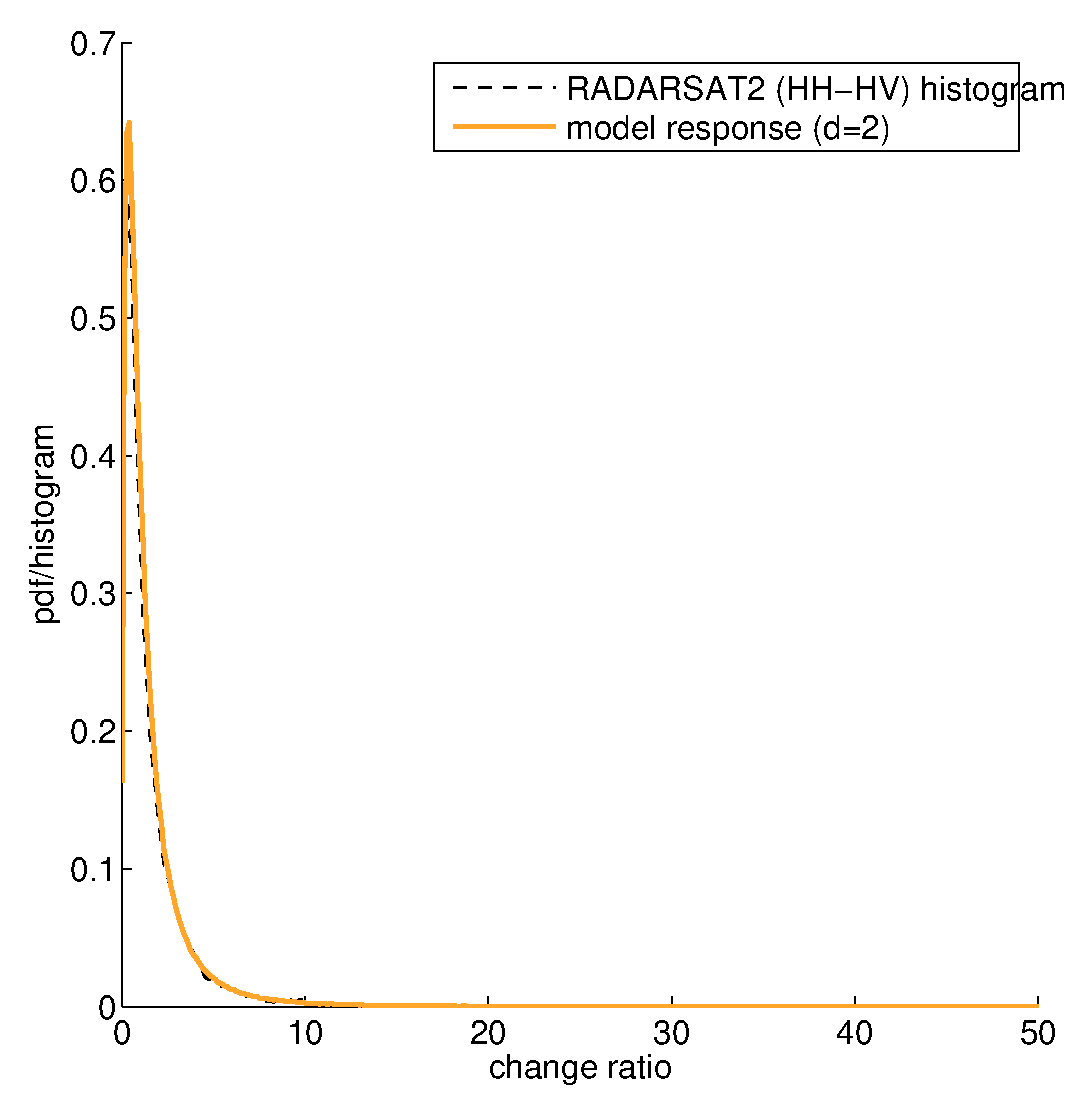
\includegraphics[width=1.5in,height=1.5in]{../images/verify_change_ratio_model_on_RADARSAT2_2d.eps}}
%          \begin{pspicture}[showgrid=false](\column,\row)% set showgrid=false for the final
%	    \rput[bl](0,0){\usebox\IBoxCRTwoR}
%	    \rput(5,1.5){\footnotesize{change-ratio}}
%	    \rput{90}(1.5,5){\footnotesize{pdf/histogram}}
%	    \psline[linecolor=plot](5,8)(6,8)
%	    \psline[linestyle=dashed](5,9)(6,9)%another line style: dotted
%	    \rput(8,8){\footnotesize{model}}
%	    \rput(8,9){\footnotesize{data}}
%          \end{pspicture}
%		 \epsfxsize=1.5in
%		 \epsfysize=1.5in
%		 \epsffile{../images/verify_change_ratio_model_on_RADARSAT2_2d.eps} 	
		 \label{RADARSAT2_2D_det_ratio}
                \subcaption{RADARSAT2 (HH-HV) change ratio}
 \end{minipage}                 
%	}
\end{tabular}
\caption{The specific $d=2$ models are validated on both RADARSAT2 and AIRSAR datasets.
Each histogram plots the signal under investigation (along the x-axis) against its probabilistic distribution across the patch (on the y-axis).}
\label{fig:verify_det_ratio_model_2D}
\end{figure}

\begin{figure}[h]
\centering
\begin{tabular}{c}
%	\subfloat[][AIRSAR (HH-HV-VV) \\ determinant]{
 \begin{minipage}[b]{1.8in} 
   \centering
          \plotWithLegend{../images/verify_determinant_model_on_AIRSAR_3d.eps}{determinant}
%		 \epsfxsize=1.5in
%		 \epsfysize=1.5in
%		 \epsffile{../images/verify_determinant_model_on_AIRSAR_3d.eps} 	
		 \label{AIRSAR_3D_determinant}
                \subcaption{AIRSAR (HH-HV-VV) determinant}
 \end{minipage}                 
%	} 
	\hfill	
%	} \\
%	\subfloat[][AIRSAR (HH-HV-VV) \\ determinant ratio]{
 \begin{minipage}[b]{1.8in} 
   \centering
          \plotWithLegend{../images/verify_det_ratio_model_on_AIRSAR_3d.eps}{determinant-ratio}
%		 \epsfxsize=1.5in
%		 \epsfysize=1.5in
%		 \epsffile{../images/verify_det_ratio_model_on_AIRSAR_3d.eps} 	
		 \label{AIRSAR_2D_det_ratio}
                \subcaption{AIRSAR (HH-HV-VV) determinant ratio}
 \end{minipage}                 
%	} 
	\hfill	
%	\subfloat[][AIRSAR (HH-HV-VV) \\ change ratio]{
 \begin{minipage}[b]{1.8in} 
   \centering
          \plotWithLegend{../images/verify_change_ratio_model_on_AIRSAR_3d.eps}{change-ratio}
%		 \epsfxsize=1.5in
%		 \epsfysize=1.5in
%		 \epsffile{../images/verify_change_ratio_model_on_AIRSAR_3d.eps} 	
		 \label{AIRSAR_2D_change_ratio}
                \subcaption{AIRSAR (HH-HV-VV) change ratio}
 \end{minipage}                 
%	}
 \\
%`	\subfloat[][RADARSAT2 (HH-HV-VV) \\ determinant]{
 \begin{minipage}[b]{1.8in} 
   \centering
          \plotWithLegend{../images/verify_determinant_model_on_RADARSAT2_3d.eps}{determinant}
%		 \epsfxsize=1.5in
%		 \epsfysize=1.5in
%		 \epsffile{../images/verify_determinant_model_on_RADARSAT2_3d.eps} 	
		 \label{RADARSAT2_3D_determinant}
                \subcaption{RADARSAT2 (HH-HV-VV) determinant}
 \end{minipage}
 \hfill
%	\subfloat[][RADARSAT2 (HH-HV-VV) \\ determinant ratio]{
 \begin{minipage}[b]{1.8in} 
   \centering
          \plotWithLegend{../images/verify_det_ratio_model_on_RADARSAT2_3d.eps}{determinant-ratio}
%		 \epsfxsize=1.5in
%		 \epsfysize=1.5in
%		 \epsffile{../images/verify_det_ratio_model_on_RADARSAT2_3d.eps} 	
		 \label{RADARSAT2_2D_det_ratio}
                \subcaption{RADARSAT2 (HH-HV-VV) det-ratio}
 \end{minipage}                
%	} \\
	\hfill	
%	\subfloat[][RADARSAT2 (HH-HV-VV) \\ change ratio]{
 \begin{minipage}[b]{1.8in} 
   \centering
          \plotWithLegend{../images/verify_change_ratio_model_on_RADARSAT2_3d.eps}{change-ratio}
%          \begin{pspicture}[showgrid=false](\column,\row)% set showgrid=false for the final
%	    \rput[bl](0,0){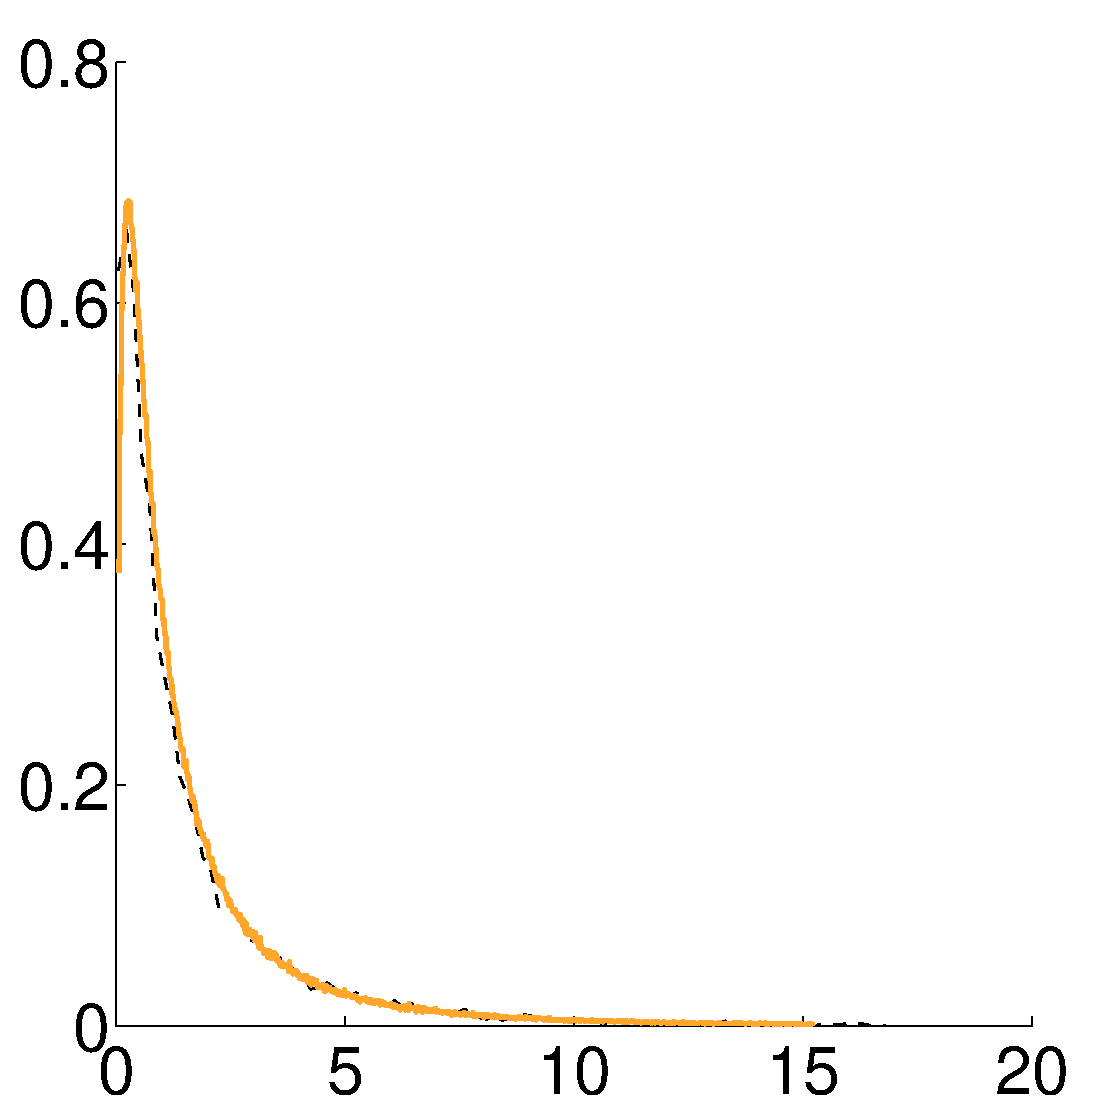
\includegraphics[width=1.5in,height=1.5in]{../images/verify_change_ratio_model_on_RADARSAT2_3d.eps}}% \usebox\IBoxCRThreeR
%	    \rput(5,1.5){\footnotesize{change-ratio}}
%	    \rput{90}(1.5,5){\footnotesize{pdf/histogram}}
%	    \psline[linecolor=plot](5,8)(6,8)
%	    \psline[linestyle=dashed](5,9)(6,9)%another line style: dotted
%	    \rput(8,8){\footnotesize{model}}
%	    \rput(8,9){\footnotesize{data}}
%          \end{pspicture}
%		 \epsfxsize=1.5in
%		 \epsfysize=1.5in
%		 \epsffile{../images/verify_change_ratio_model_on_RADARSAT2_3d.eps} 	
		 \label{RADARSAT2_2D_change_ratio}
                \subcaption{RADARSAT2 (HH-HV-VV) change ratio}
 \end{minipage}                 
%	}
\end{tabular}
\caption{The specific $d=3$ models are validated on both RADARSAT2 and AIRSAR datasets.
Each histogram plots the signal under investigation (along the x-axis) against its probabilistic distribution across the patch (on the y-axis).}
\label{fig:verify_det_ratio_model_3D}
\end{figure}

%***IVM: SIMPLY COMMENT OUT THE DISCUSSION, MOVE ANY IMPORTANT ASPECTS TO THE CONCLUSION
%\section{Discussion}
%\label{sec:discussion}
%
%%Let us begin by noting
%To begin, a few theoretical properties of the proposed statistical models are discussed.
%First, the use of covariance matrix log-determinant may be related to the standard eigen-decomposition method of the POLSAR covariance matrices.
%In fact, the log-determinant can also be computed as the sum of log-eigenvalues.
%Specifically $\ln{|M|} = \sum \ln{\lambda_M}$ where $\lambda_M$ denotes all the eigenvalues of $M$.
%Thus, similar to other eigenvalue based approaches (e.g. entropy/anisotropy, ...),
%  the models presented here are invariant to polarization basis transformations.
%
%Second, the models are developed for the POLSAR covariance matrix.
%However, since the POLSAR coherency matrix is related to the covariance matrix via a unitary transformation which preserves the determinant,
%  the model is also applicable to the coherency matrix.
%
%It should be noted that despite these advantages, the model descriptions are far from complete.
%While it is desirable to reduce the multi-dimensional POLSAR data to a scalar value for many applications,
%  such a reduction is unlikely to be lossless.  
%Ideally %to better understand POLSAR data
%the use of this technique could be complemented by some high-dimensional POLSAR target-decomposition techniques, such as the Freeman Durden decomposition \citep{Freeman_1998_TGRS_963} or the entropy/anisotropy decomposition \citep{Cloude_1997_TGRS_68} or similar.
%
%Nevertheless the proposed models are promising.
%Even though initially developed for partial and monostatic POLSAR data,
%  it was shown to be applicable to traditional SAR data as well.
%Since the model assumptions are quite minimal, they may potentially be applicable to bi-static and interferometric data, although that would require further study.
%
%Intuitively, the concept of the determinant being representative of the POLSAR data can be thought of as being similar to the concept of using the magnitude to represent a complex number
%(in a sense this is also why intensity is widely considered representative of the complex SAR data).
%Similar to the determinant, the magnitude observable is also scalar and is not lossless, but it is undeniably useful.
%To fully represent the complex number, another observable would needed besides the magnitude, for example a polar representation.
%Magnitude is, of course, widely used as it can be shown to be invariant to a change in the reference frame.
%Similarly, the determinant of the POLSAR covariance matrix is also scalar and invariant to a change of polarization basis.
%Thus while it may not be \textit{fully} representative of the POLSAR data, it can be said to be \textit{highly} representative of it.
%The important point is that it can provide a scalar comparison of the multi-dimensional data.
%%**IVM removed this This is similar to the most commonly used magnitude to compare two or more complex numbers. %, most of the times the magnitude is to be used. 
%
%Besides the above properties, the theoretical models may also provide an alternative derivation for the likelihood test statistics widely used in POLSAR.
%Similar to the way that different measures of distance can be used to derive POLSAR classifiers \citep{Lee_1999_TGRS}, change detectors \citep{Conradsen_2003_TGRS_4}, edge detectors \citep{Schou_2003_TGRS_20} or other clustering and speckle filtering techniques \citep{Le_2010_ACRS} \citep{Le_2011_ACRS}, 
%new detection, classification, clustering or speckle filtering algorithms can be derived using the models presented in this paper.
%These applications however are not included in this paper, but rather left as a suggestion for future investigations.

\section{Conclusion}
\label{sec:conclusion}

%What has been done?
This paper has proposed a generic statistical model  for the POLSAR covariance matrix determinant based on the complex Wishart POLSAR target vector distribution.%***IVM: Hai pls check this sentence!
This model has been validated for specific ($d=2$) and ($d=3$) using real-life partial and full POLSAR data.
The paper also establishes a few POLSAR discrimination measures: the determinant-ratio and the change-ratio,  which essentially are the generic version of the SAR intensity-ratio.
We have also shown a near-perfect match between the specific $d=1$ model and that for traditional SAR intensity,
  effectively bringing the existing SAR theories under the umbrella of this new model.

%What are the results? What are their advantages over others' results?
The main emphasis of this paper is the proposal to consider the POLSAR covariance matrix determinant as a scalar and representative observable for the multi-dimensional POLSAR data.
Compared to other published scalar observables, the determinant is highly representative of the multi-dimensional data.
It is also invariant to a change of polarization basis.
While it may not be \textit{fully} representative of the POLSAR data, it can be said to be \textit{highly} representative of it.
Its representative power is justified for the following reasons.
Firstly, the covariance matrix determinant, when collapsed into 1-D, transforms neatly into the representative SAR intensity.
Secondly, the statistical model for this observable is shown to be the generic multi-dimensional extension of the traditional model for the one dimensional SAR intensity.
Finally, this observable also leads to the establishment of the determinant-ratio discrimination measure for POLSAR data, which should increase the usability of this proposal.

%What are their benefit?
There are several beneficial implications of the proposed approach presented in this paper.
Currently while the field of SAR is much more developed than the field of POLSAR,  the two fields remain  quite separated.
Hence many techniques applicable to SAR can not be directly translated to POLSAR.
Since the scalar and representative model for POLSAR generalizes the traditional model for SAR intensity,
  its main benefit is that it enables the convenient adaptation of many existing SAR data processing techniques for POLSAR data.
One example has already been presented in this paper, 
  where existing SAR discrimination measures are extended towards POLSAR.
At the same time, it provides a consistent theory unifying the seemingly disparate discrimination measure proposals for SAR and POLSAR data.  

%What are their limitations? What problems this appears to solve, but actually is not?
Of course, the models proposed in this article also have their own limitations.
Firstly, they are based on the complex Wishart distribution
%Thus its applicability is also limited by that of its foundation,
%  that is the proposed theoretical model 
  which is only guaranteed to work for homogeneous areas.
Secondly, while it is desirable for a large number of applications to reduce the multi-dimensional POLSAR data to a scalar value, such a reduction is unlikely to be lossless in the general case.

In this paper, the theoretical model has only been validated for partial ($d=2$) and full ($d=3$) monostatic POLSAR data,
%and hence What can be done next?
  leaving the test of its validity for datasets such as bistatic POLSAR data ($d=4$) or interferrometric POLSAR data ($d=6$) for the future.
Other possible extensions include
  investigating the applicability of the observables into POLSAR heterogeneous areas,
  as well as exploring the use of these generic models in conjunction with other target decomposition techniques
    such as the Freeman-Durden decomposition \citep{Freeman_1998_TGRS_963} or the entropy/anisotropy decomposition \citep{Cloude_1997_TGRS_68}.

% references section
\bibliographystyle{tRSL}
\bibliography{paper}

\end{document}

